\section{コードリーディング支援システムの開発}

本項では,プログラミング初学者を対象としたコードリーディング支援システムについて紹介し,設計指針に基づくデザインの詳細,プロトタイプを用いたケーススタディとその後に開発したWebアプリケーションについて説明する.

\subsection{研究背景}
プログラミングの重要性の高まりに伴い,コンピュータに関連する分野を専攻していなくとも,プログラミングを独学で学ぼうとする人が増えている.そういった人はプログラミング学習用書籍やWebサイトを通して学ぶ場合が多い.初学者向けプログラミング学習コンテンツが普及し,プログラミングに入門するハードルは下がってきているものの,まだプログラミングを独習できる環境が整っているとは言えない.

プログラミング学習において重要とされるスキルは数多くあり,自分でアルゴリズムを考え実装する能力だけでなく,情報収集能力,コードリーディングスキルなど様々である.これらをコンピュータについての知識が乏しい者が独習するのはハードルが高い.初学者向け学習教材においては,写経型学習を主とし,プログラムを「書く」技能を磨かせるものが多い.プログラミング学習サイトであるProgate\cite{progate}では,主要なプログラミング言語の文法やライブラリの用法など,「どうプログラムを書くか」を重点的に教えている.


しかし学習教材を用いた学習では,コードを「読む」技能,すなわちコードリーディングスキルが培われず,複数人で共同開発し他人の記述したプログラムを読解したり,ライブラリのソースコードにあたる際に苦労が生じる.また初学者向け学習教材では比較的平易なプログラムしか載っていないため,実践的なソースコードに触れ,内容を読解したり,他者のコーディングスタイルから学びを得る機会が生まれ辛い.

本項で提案するシステムでは,コードリーディングスキルに焦点を当て,エンタテインメントの要素を組み込んで初学者に実践的なプログラムを閲覧させることにより,初学者のコードリーディングを促進するシステムを実装した.
\subsection{関連研究}

%GitHub使った研究
\subsubsection{GitHub上のデータを利用した研究}
GitHubを活用した研究はいくつかある.Guzmanらの研究ではGitHub上のオープンソースプロジェクトにおけるコミットコメントから感情分析をし,その結果とプログラミング言語やコミットの時間などとの相関を調査している\cite{guzman}.永野らの研究ではGitHubとStackOverflowのデータを用いて双方を利用するユーザについて調査している\cite{nagano}.この研究ではユーザがGitHubで作成したリポジトリとStackOverflowへの投稿のコンテンツの関連性について調べたもので,双方への投稿コンテンツに一定の相関があることを示している.また柴藤らはGitHub上の断片データに関する情報を取得できるシステムを開発している\cite{shibatou}.このシステムではユーザが指定したソースコード中の一部の連続したコードに関するプルリクエストを取得できるというものであり,ソースコードを閲覧する際の利便性を高めている.これらの研究からGitHubのソースコードやコミットコメントには有益な情報が含まれていることが分かるが,これらを初学者のコードリーディング支援のために活用している例は見かけない.

%エンタテインメント,ゲーミフィケーション使った研究
\subsubsection{ゲーミフィケーションを活用した研究}
またエンタテインメントの要素,特にゲーミフィケーションを活用した研究も盛んである.一ノ瀬らの研究\cite{ichinose}ではソースコード上の技術的負債を可視化し,さらにゲーミフィケーションの要素を加えることで技術的負債の除去を促している.この研究ではソースコードのファイル構造を街のように可視化し,技術的負債が存在するファイルを目立たせ,さらに技術的負債を取り除いたユーザをランキング形式で表示することによって,ゲーミフィケーションの要素を活用し生産的な行動を促している.三谷らの研究\cite{mitani}ではキャラクタをプログラムで制御するプログラミングゲームでプログラミングスキルの向上を図っており,筒井らの研究\cite{tsutsui}ではパズルゲームにより,初学者のオブジェクト指向の理解を深めるシステムを開発している.これらはプログラミングの上達あるいはソフトウェア開発のためにゲーミフィケーションを利用しているが,コードリーディングに着目し,初学者のコードリーディングを促進するためにゲーミフィケーションを利用したシステムは見かけない.

%コードリーディングに関する研究
\subsubsection{コードリーディング支援に関する研究}
なおコードリーディング支援に関してもいくつか研究がなされており,大村らや石尾らはソースコードを読解する際のコードリーディング支援を行うツールを開発している\cite{omura}\cite{ishio}.
しかし,これらの研究ではある程度プログラミングに習熟したプログラマがソースコードを読むという状況を想定しているため,初学者に向けコードに触れる機会を増やすための工夫は成されていない.
\subsection{設計指針}
システムを実装するにあたり,研究指針に基づいた3つの設計指針を設けた.
\begin{enumerate}
  \item {\bf クイズ・占いを用いる}

  コードリーディングはプログラミングにおいて重要なスキルの1つであるが,プログラムを読解した経験の少ないプログラミング初学者にとって,淡白なプログラムをただ読み込むことは心理的ハードルが高い.よって本システムではクイズ・占いといった誰もが知っているエンタテインメントの要素を付与してプログラムを読解させ,コードリーディングの心理的障壁を下げることを目指した.


  \item {\bf プログラムを読んで楽しめる}


  本項で述べるシステムの目的は,初学者のコードリーディングを促進することである.プログラムを「書く」ことに焦点をおいた教材は他に多く存在するため,本システムではプログラムを「読む」ことのみに専念させ,余計な認知的負荷をかけずに読解に集中できるように設計する.また1つのプログラミング言語を読解するだけでなく,様々なプログラミング言語に触れることで,コンピュータを取り巻くプログラミング言語とそのライブラリ,エコシステムなどに触れ,プログラミングに対する興味関心を高めることが可能であると考え,1つのプログラミング言語のみを対象とした機能と様々なプログラミング言語に触れる機能を用意した.


  \item {\bf コミュニケーションを創出する}
  
  初学者がプログラミングを独習する場合,プログラミングを学習している者とのコミュニケーションが発生しづらく,モチベーションが下がる場合がある.本項で提案するシステムでは,エンタテインメントの要素を用いるだけでなく,初学者同士あるいは初学者とプログラマのプログラミングに関するコミュニケーションのきっかけを与え,楽しく継続的なシステムの利用を促す.
\end{enumerate}

\subsection{提案システム}
\subsubsection{実装機能}
提案システムに実装する,エンタテインメントの要素を用いた2つの機能について説明する.
\begin{itemize}
  \item {\bf クイズ機能}

  この機能はユーザが使用した際にGitHubからランダムに取得したプログラムを表示する.プログラムの記述言語は多様であり,ユーザは表示されたプログラムを読み,どのプログラミング言語で記述されたプログラムかを回答する.正解した場合は得点が得られ,取得した累計得点の多さによるランキングが表示される.設計指針2で述べた様々な言語に触れられる機能に相当する.

  \item {\bf 占い機能}

  この機能をユーザが使用するとGitHubからランダムに得られたプログラムが表示され,ユーザはそれを読解し自分なりの解釈をすることで,その日の運勢を占う.表示されたソースコードの意味を解釈することが必要であるため,必然的にコードの読解が必要となる.この機能においては表示されるプログラムをJavaScriptで記述されたものに限定した.

\end{itemize}

\subsection{プロトタイプシステム}
初めに,提案システムをチームコミュニケーションツールであるSlackのbotとして実装した.システムを利用する際は,このbotを導入しているチャンネルでコマンドを入力することで各機能を使用できる.利用可能なコマンドを表\ref{function}に示す.

また表示するプログラムは内容が1つのファイルにまとまっていることが望ましいため,GitHub Gistからプログラムを取得した.クイズ機能を使用している様子を図\ref{prototype_quiz}に,占い機能を使用している様子を図\ref{prototype_fortune}に示す.

\begin{table}[!ht]
  \centering
    \caption{コマンド一覧}
      \begin{tabular}{|c|c|} \hline
        コマンド & 説明 \\ \hline \hline
        fortune & 1日の運勢を占うソースコードを表示 \\ \hline
        quiz & 記述言語を問うクイズを出題 \\ \hline
        hint & クイズに関するヒントを表示 \\ \hline
        answer & クイズの回答を表示 \\ \hline
        score & 各ユーザの累計得点を表示 \\ \hline
      \end{tabular}
    \label{function}
  \end{table}

\begin{figure}[!h]
  \begin{center}
    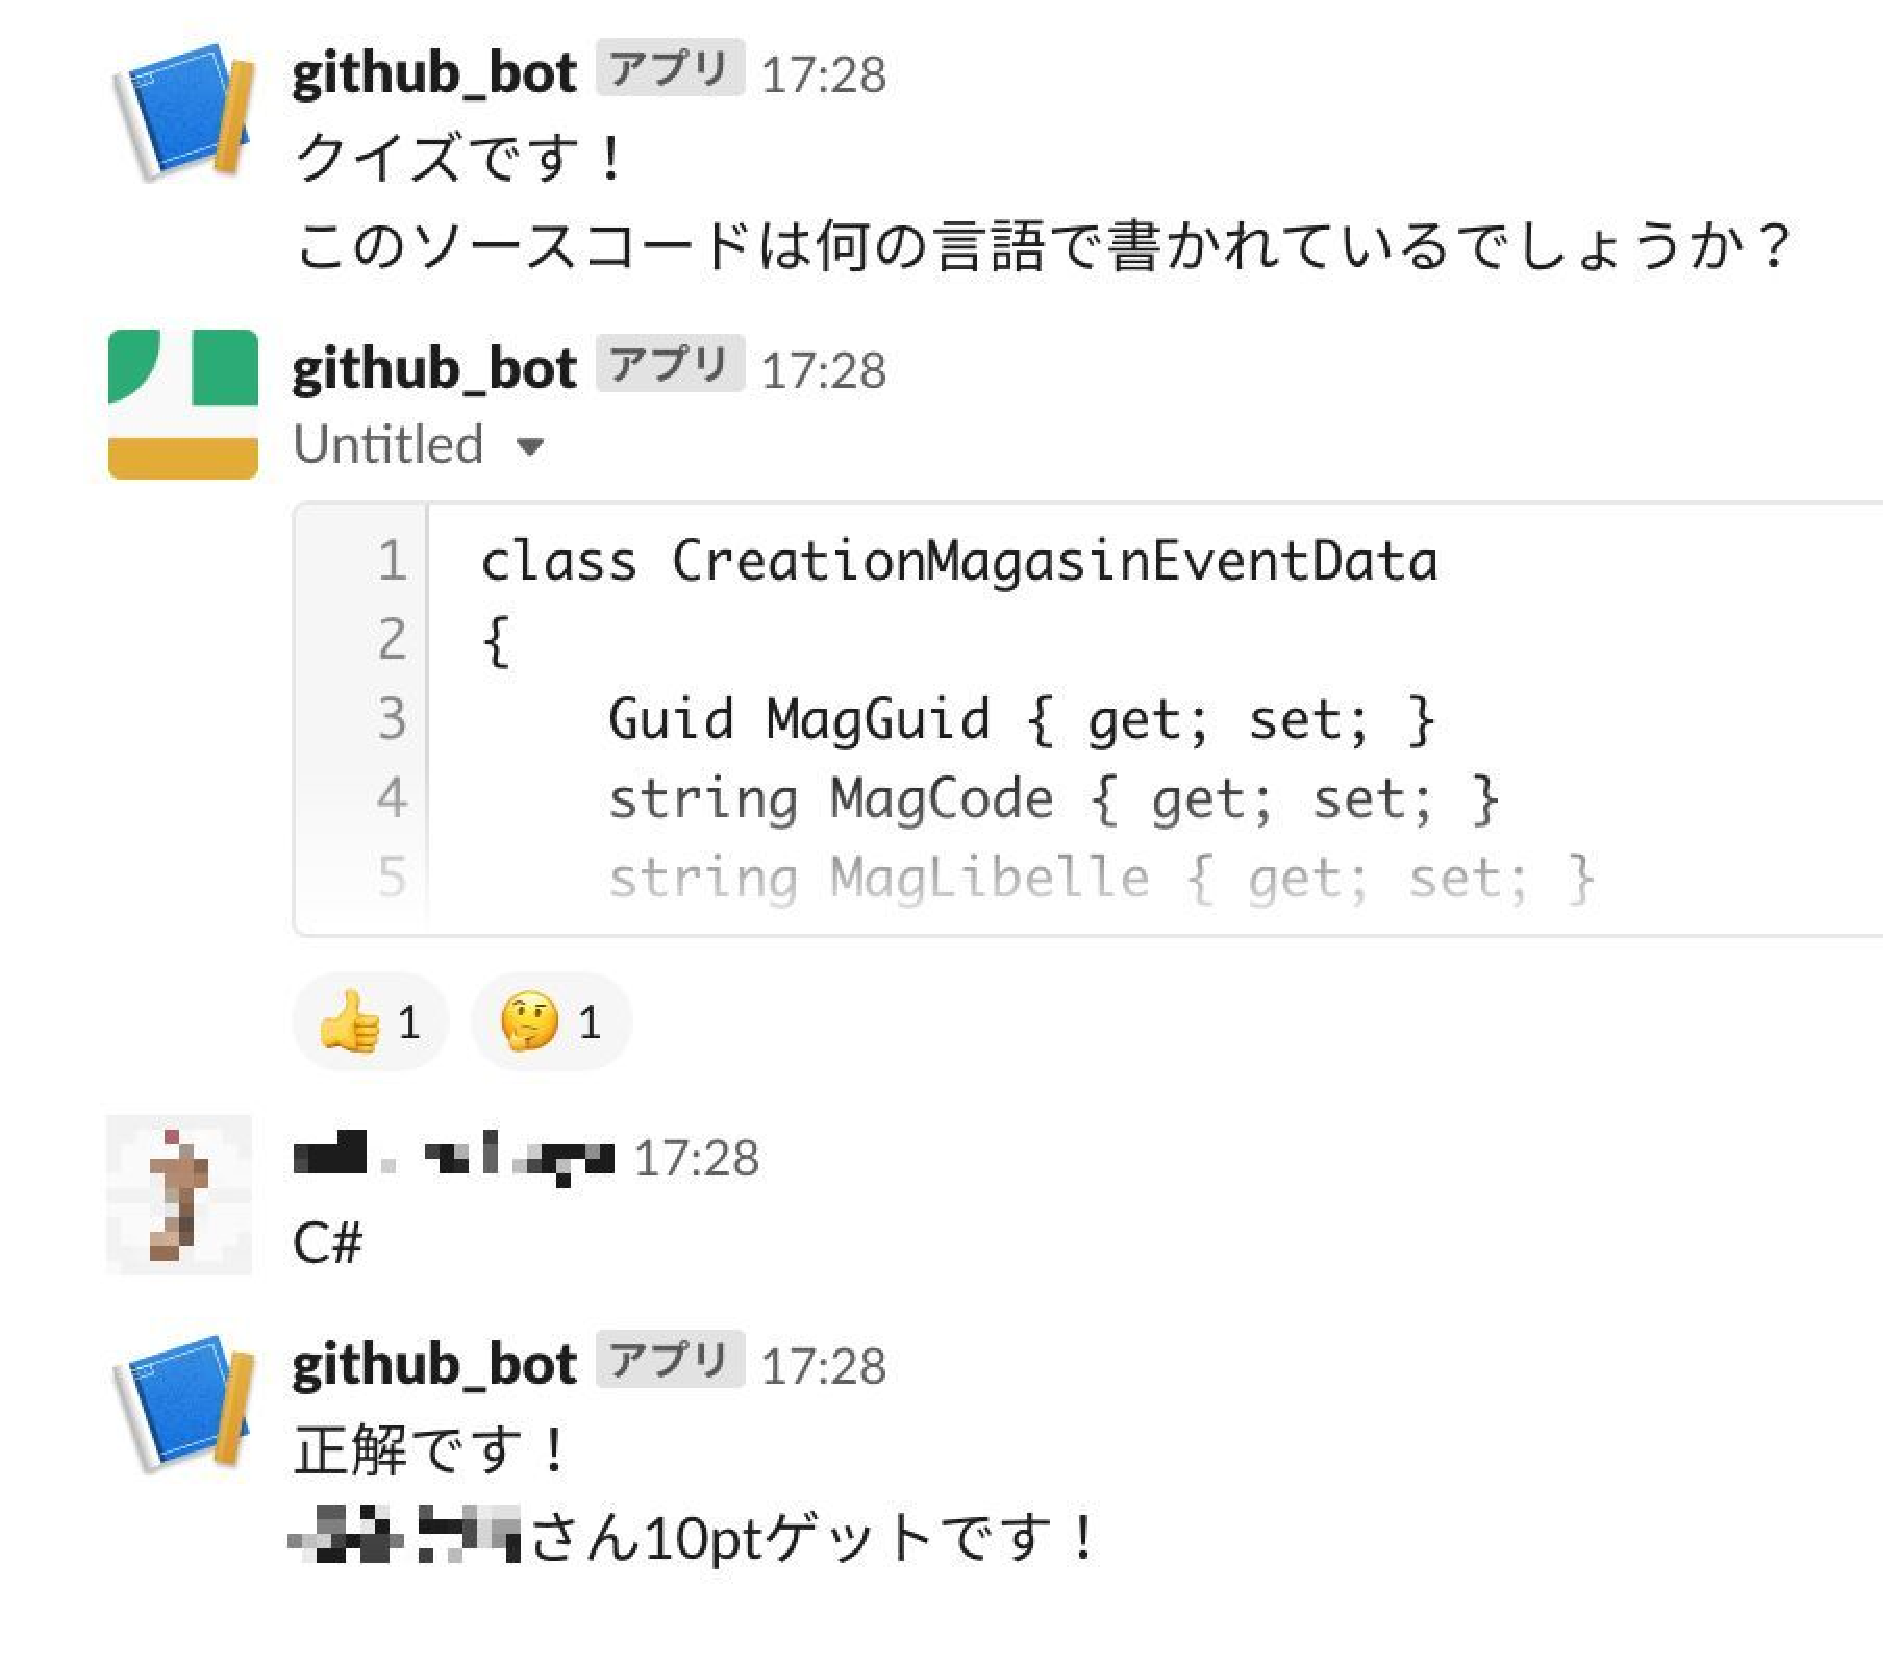
\includegraphics[width=0.4\linewidth]{image/prototype_quiz.eps}
  \end{center}
    \vspace{-8mm} 
  \caption{クイズ機能の様子}
  \label{prototype_quiz}
\end{figure}

\begin{figure}[!h]
  \begin{center}
    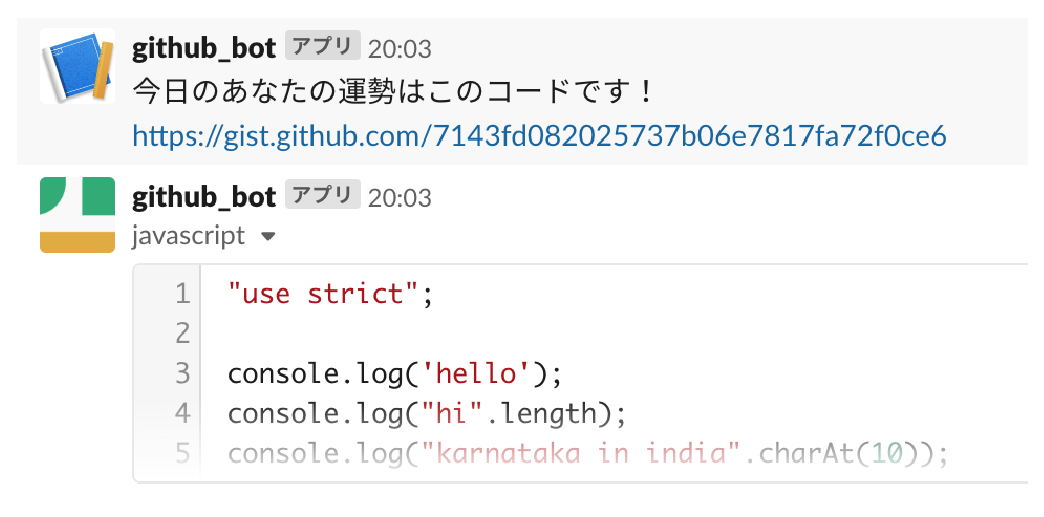
\includegraphics[width=0.6\linewidth]{image/prototype_fortune.eps}
  \end{center}
    \vspace{-8mm} 
  \caption{占い機能の様子}
  \label{prototype_fortune}
\end{figure}


\subsubsection{ケーススタディ}
このシステムを筆者が所属する研究室で運用しているSlackのチャンネルに導入し,システムの効果を調査するため,研究室のメンバーを対象としたケーススタディを行った.研究室のメンバーは3名のプログラミング初学者であり,主にJavaScrtipやGoogle Apps Scriptを使用している.ケーススタディの内容としては,1週間自由に機能を使用してもらい各コマンドの使用回数を調べ,アンケートによって所感を調査した.アンケートの項目を以下に示す.

\begin{itemize}
  \item どういう状況で機能を使用したか
  \item 占い機能について,楽しかったか(5段階評価,1:楽しくなかった,5:楽しかった)
  \item 占い機能について,どういう点が楽しかった(楽しくなかった)か
  \item クイズ機能について,楽しかったか(5段階評価,1:楽しくなかった,5:楽しかった)
  \item クイズ機能について,どういう点が楽しかった(楽しくなかった)か
  \item 機能を使用したことによって学びがあったか
  \item どういう学びがあったか
  \item コードを読むことへの抵抗は減ったと感じるか(5段階評価,1:減らなかった,5:減った)
  \item 今後も機能を使いたいか
  % \item 感想,意見,改善点など
\end{itemize}

また各コマンドの使用回数を表\ref{command}に示す.

\begin{table}[!h]
  \centering
  \caption{各コマンドの使用回数}
  \label{command}
    \begin{tabular}{|c|c|} \hline
      コマンド & 使用回数 \\ \hline \hline
      fortune & 9 \\ \hline
      quiz & 43 \\ \hline
      hint & 27 \\ \hline
      answer & 3 \\ \hline
      score & 33 \\ \hline
    \end{tabular}
\end{table}

コマンドの使用回数に関しては,クイズ機能に関連した機能が多い結果となり,占い機能に関しては使用回数が少なかった.なお期間中の最初の3日間ほどは頻繁にシステムが使用されていたが,期間の後半おいてはあまり活発に使用されていなかった.またどの機能も個別に使用するより,ユーザが実際に会って集まっている際にコミュニケーションを交えて使用されることが多く,コミュニケーションを促進できていたと考えられる.

次にアンケート結果を表\ref{interview}に示す.
\begin{table}[!b]
  \centering
  \caption{アンケート結果}
  \label{interview}
    \begin{tabular}{|c|c|c|c|} \hline
      インタビュー内容 & 被験者A & 被験者B & 被験者C \\ \hline \hline
      占い機能は楽しかったか & 1 & 2 & 3 \\ \hline
      クイズ機能は楽しかったか & 4 & 4 & 5 \\ \hline
      コードへの抵抗感は減ったか & 3 & 5 &5 \\ \hline
    \end{tabular}
\end{table}

まず占い機能に関してだが,使用する楽しさの評価は低い結果となった.ユーザの意見には「提示されたプログラムをどう解釈すればいいのか分からなかった」「占いという感触があまりなかった」などがあり,プログラミング初学者にとってプログラムを読解して独自の解釈を持たせることは難しく,面白みに欠けているようだった.

またクイズ機能に関しては楽しさに関して高い評価が得られた.その理由として「スコアがあると、競争している感が出るところが楽しく感じた」「みんなで一緒にやっていて競争っぽくなるとき楽しかった」などの意見があり,スコアを用いたゲーミフィケーション,競争の要素がシステム使用のモチベーションを高めていたと考えられる.

なお「以前に出た言語の特徴に似ていると感じ、調べずに答えて正解したとき楽しかった」という意見が得られ,クイズを通したコードリーディングによってプログラミング言語の特徴を捉え,それに楽しみを感じていることが分かった.

「機能を使用したことによって学びがあったか」という質問には全員が「あった」と回答し,「どういう学びがあったか」という質問には「言語ごとの文法の特徴が何となく分かってきた」「いろんな言語の存在を知ることができました」「今まで聞いたこともなかったプログラミング言語の名前を知り、親近感をもった」という回答があり,各プログラミング言語の特徴について理解するとともにプログラミングに対する親近感を抱かせることができていた.

またプログラムへの抵抗感に関する質問でも肯定的な評価が得られ,「今後も機能を使いたいか」という質問に対して全員が「使いたい」と回答した.なおシステムの改善点に関して「プログラムのあるGitHubのページへのリンクを表示して欲しい」「占いの際にラッキーアイテムなどを表示して欲しい」等の意見が得られたため,アンケート結果を元にプロトタイプを改善したシステムを開発した.

\subsection{Webアプリケーション}
プロトタイプシステムを用いたケーススタディで得られた結果を元に,プロトタイプシステムを改善し,Webアプリケーションとして再実装した.Webアプリケーションとして実装したのはSlack botよりも開けたコミュニティでより多くのユーザの意見を取り入れるためである.

このアプリケーションでは指定のURLにアクセスすることでクイズ・占いの機能を使用でき,ユーザ登録をしログインすることでクイズ正解時に得た得点の累計によるユーザのランキングを閲覧することができる.またクイズ機能においてはそのクイズに対するユーザの正答率,占い機能においては選ばれたプログラムに含まれているコメントの量,宣言された関数の数などから独自に算出した対人運,仕事運,コメントなどを表示するようにした.クイズ機能の様子を図\ref{quiz}に,占い機能の様子を図\ref{fortune}に示す.

\begin{figure}[H]
  \begin{center}
    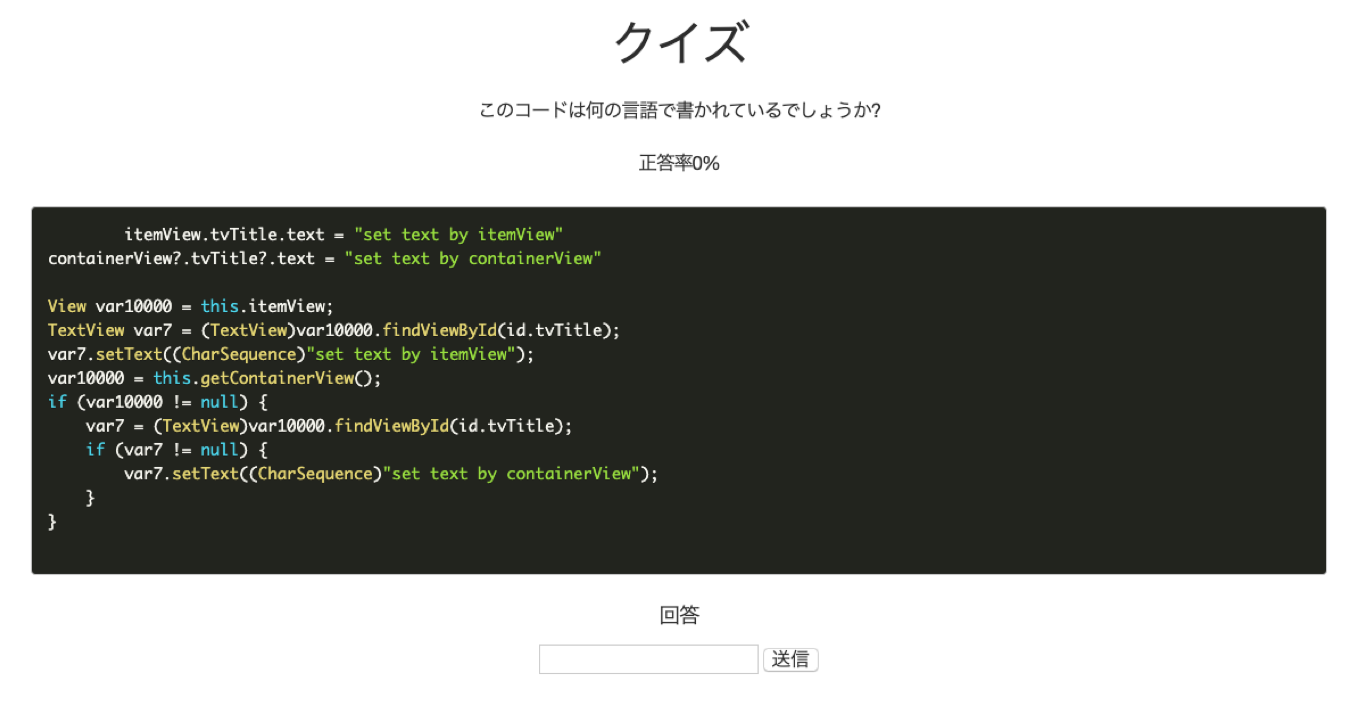
\includegraphics[width=0.8\linewidth]{image/quiz.eps}
  \end{center}
    \vspace{-8mm} 
  \caption{クイズ機能の様子}
  \label{quiz}
\end{figure}

\begin{figure}[H]
  \begin{center}
    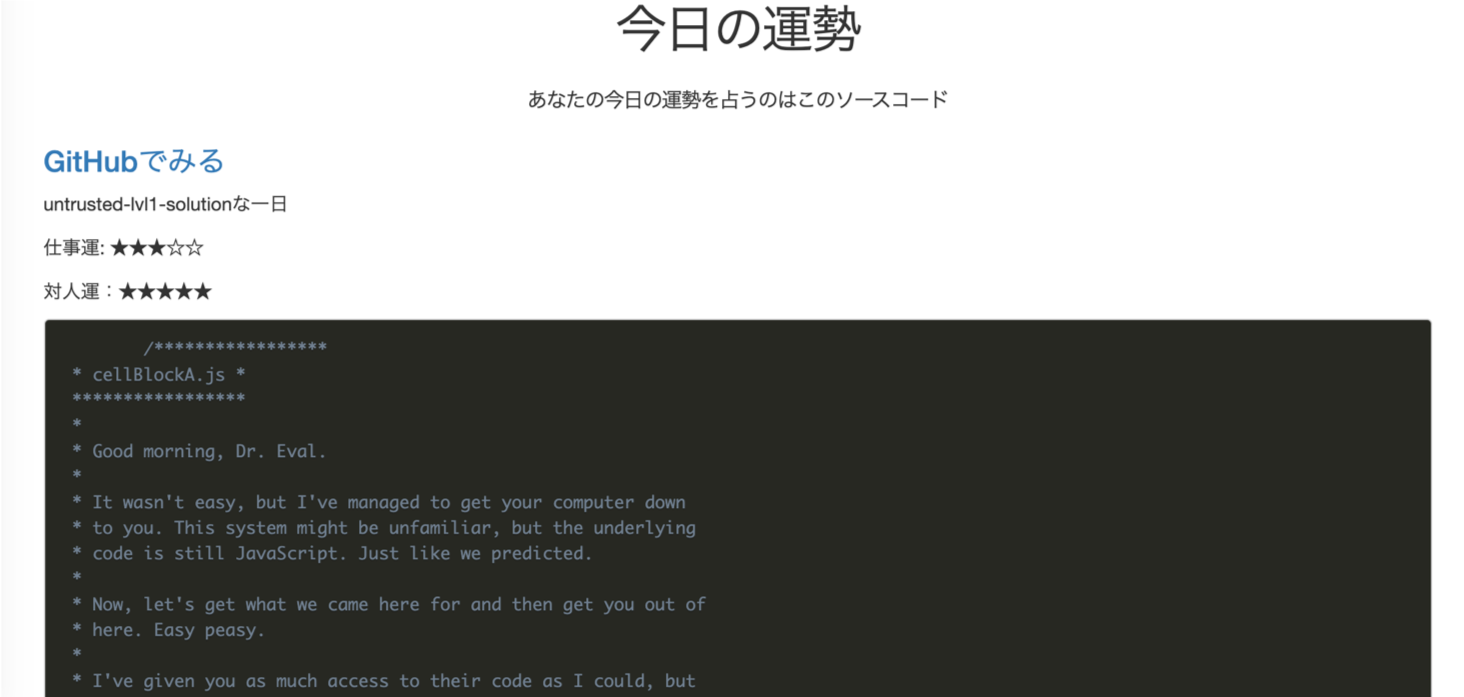
\includegraphics[width=0.8\linewidth]{image/fortune.eps}
  \end{center}
    \vspace{-8mm} 
  \caption{占い機能の様子}
  \label{fortune}
\end{figure}

また実装したアプリケーションをUbiquitous Wearable Workshop2019\cite{uww2019}にて参加者に使用させ,議論を行った.占い・クイズ機能ともに使用され,表示されたプログラムを見せ合うなどシステムを介したコミュニケーションが見られたが,「クイズが難しすぎて逆にプログラムに対する抵抗感が生まれた」というコメントもあった.




\subsection{課題と考察}

提案システムのプロトタイプ及びそれを元にしたWebアプリケーションの実装と運用を通して,エンタテインメントの要素やコミュニケーションの要素,特にクイズの要素を交えてプログラミング初学者のコードリーディングを促進することは,有効な方策であると考えられる.またその中で他者と競争するゲーミフィケーションはシステムを使用するモチベーションとなり,これをプログラミング学習コンテンツに取り込むことで有益な学習コンテンツを作成できると感じた.しかし,現状実装したアプリケーションには不十分な箇所が多く,より適切なゲームデザイン,ユーザがシステムを使い続けるための工夫,どのようなアルゴリズムでプログラムを選び,初学者に提示するかなど課題は多い.

今後はこのシステムを通して得られた課題・観点を元に,より良いプログラミング学習コンテンツを作成していく.またアンケート調査に止まらず,ユーザのコードリーディングに関する行動の追跡的な調査をし,システムに関する客観的な評価を行っていきたい.
